\documentclass[UTF8, a4paper]{ctexart}
\usepackage[margin=1in]{geometry} % 页边距调整
\usepackage{ctex}
\usepackage{array, amsmath, amssymb}

\usepackage{booktabs, tabularx, multirow, multicol} % 表格拓展支持
\usepackage{graphicx, subfigure, float} % 图片排版支持

\usepackage{algorithm, algpseudocode} % 伪代码支持
\renewcommand{\algorithmicrequire}{\textbf{Input:}}  
\renewcommand{\algorithmicensure}{\textbf{Output:}} 

\usepackage{tikz, mathpazo} % 基本绘图支持
\usepackage{flowchart} % 流程图支持
\usepackage{pgf-umlcd} % UML类图支持
\usetikzlibrary{arrows, shapes, chains, shapes.geometric}

\usepackage{listings} % 代码块支持
\usepackage{xcolor}
\lstset{
	language		= c++,
	backgroundcolor	= \color{white},
	basicstyle		= \footnotesize\ttfamily,
	keywordstyle	= \color{blue},
	stringstyle		= \color{red!58!blue!82}\ttfamily,
	commentstyle	= \color{darkgray},
	rulesepcolor	= \color{red!20!green!20!blue!20},
	columns			= fullflexible,
	breaklines		= true,
	captionpos		= b,
	tabsize			= 4,
	frame			= single,
	escapeinside	= {\%*}{*)}
}
%%示例
% \begin{lstlisting}[caption={}]
% #include <iostream>
% int main(int argc, char *argv[]) {
% 	std::cout << "Hello World!" << std::endl;
% 	return 0;
% }
% \end{lstlisting}

\usepackage{datetime} %日期
\renewcommand{\today}{\number\year{年}\number\month{月}\number\day{日}}

\begin{document}

\begin{center}
	\zihao{3}《数据结构》实验报告
\end{center}
\zihao{5}

\newcolumntype{Y}{>{\raggedleft\arraybackslash}X}
\noindent\begin{tabularx}{\textwidth}{XcY}
	  {班 级:}\;\underline{DL062123}
	& {姓 名:}\;\underline{项乔栋}
	& {学 号:}\;\underline{2021302468} \\
	  {邮 箱:}\;\underline{13282135976@sina.cn}
	& {日 期:}\;\underline{\today}
	& {编 号:}\;\underline{DS02}
\end{tabularx}
~\\

\noindent\textbf{$\circledcirc$
实验题目:\quad{高精度计算$\pi$值}} \par
\noindent\textbf{$\circledcirc$
实验目的:\quad{双向链表的实际应用}} \par
\noindent\textbf{$\circledcirc$
实验内容:\quad{基于双向链表实现高精度计算并以此计算$\pi$值}} \par

\subsection*{一、需求分析}
\noindent\fbox{
\begin{tabularx}{\textwidth}{lY}
\bf{Description}
& \parbox[t]{\linewidth}{
	限制使用双向链表作存储结构,请根据用户输入的一个整数(该整数表示精确到小数点后的位数,可能要求精确到小数点后500位),高精度计算$\pi$值。可以利用反三角函数幂级展开式来进行计算。
} \\

\bf{Input}
& \parbox[t]{\linewidth}{
	输入的一个正整数$n$
} \\

\bf{Output}
& \parbox[t]{\linewidth}{
	输出$\pi$的值,精确到小数点后$n$位,最后输出一个回车
} \\

\bf{Sample Input}
& \fbox{\parbox[t]{\linewidth}{\bf{
	\mbox{5}
}}} \\

\bf{Sample Output}
& \fbox{\parbox[t]{\linewidth}{\bf{
	\mbox{3.14159}
}}}
\end{tabularx}}

\subsection*{二、概要设计}
在达成实验目的的前提下,考虑直接实现大数计算的子集,进行结构化设计,以便于后期维护、调试与优化。 \par
1.\;基本操作: \par
	Decimal(precision, InitialValue) $\rightarrow$ Decimal \par
	\qquad\textbf{操作结果:}\;以指定小数精度和初值构造大数对象 \par
	$\sim$Decimal() $\rightarrow$ void \par
	\qquad\textbf{操作结果:}\;销毁大数对象 \par
	Clone(decimal) $\rightarrow$ Decimal \par
	\qquad\textbf{操作结果:}\;拷贝大数对象 \par
	Add(lhs:Decimal,rhs:Decimal|Integer) $\rightarrow$ Decimal \par
	\qquad\textbf{操作结果:}\;大数加法的结果值 \par
	Multiply(lhs:Decimal,rhs:Integer) $\rightarrow$ Decimal \par
	\qquad\textbf{操作结果:}\;大数乘法的结果值 \par
	Divide(lhs:Decimal,rhs:Integer) $\rightarrow$ Decimal \par
	\qquad\textbf{操作结果:}\;大数除法的结果值 \par
	Output(decimal) $\rightarrow$ void \par
	\qquad\textbf{操作结果:}\;输出大数对象 \par
	CalculatePI(precision) $\rightarrow$ Decimal \par
	\qquad\textbf{操作结果:}\;计算指定小数精度的$\pi$值 \par
2.\;程序模块: \par
1) 主程序 \par
2) IO支持 \par
3) Decimal大数类 \par
\begin{figure}[H]
	\begin{minipage}[t]{\linewidth}
		\centering
		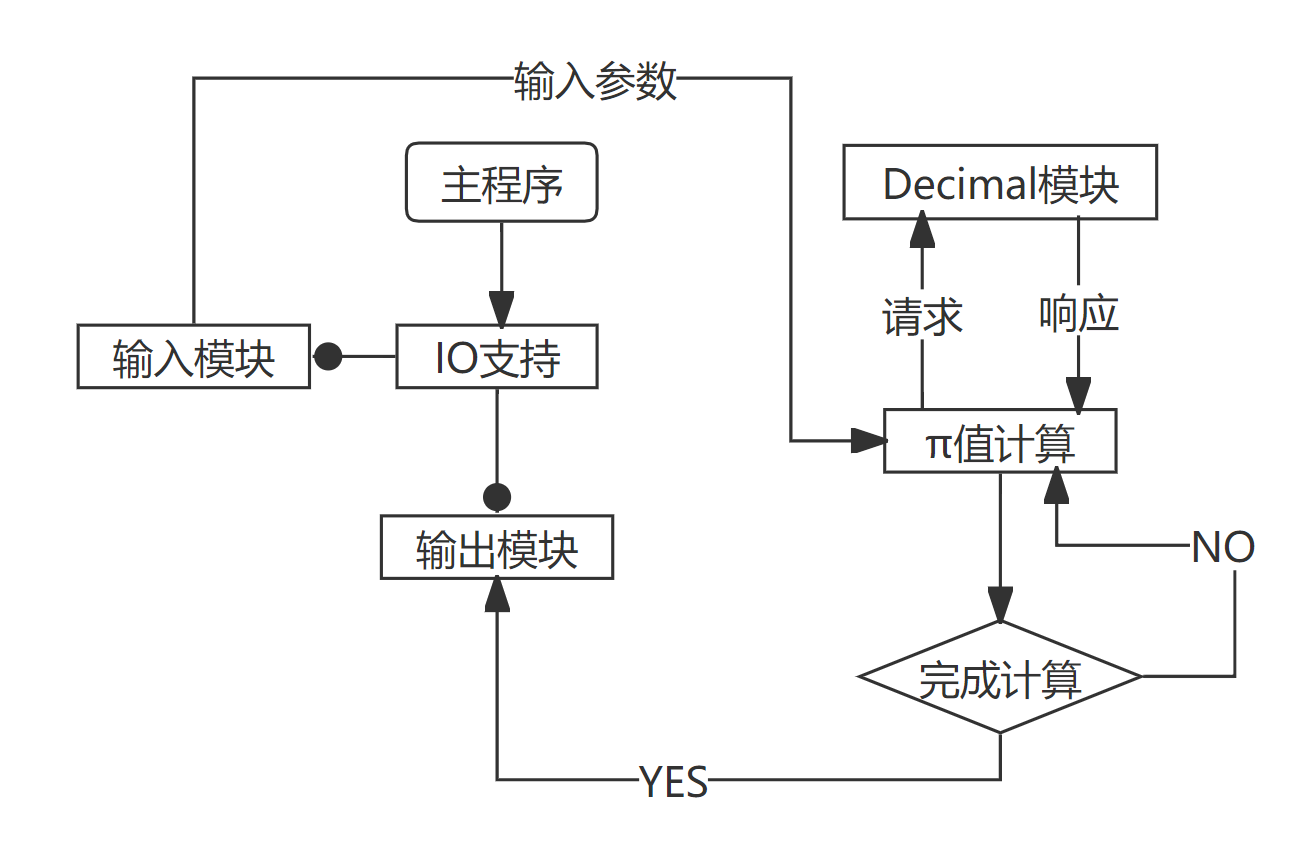
\includegraphics[width=125mm,height=80mm]{./assets/DS02-1}
	\end{minipage}
\end{figure}

\subsection*{三、详细设计}
\begin{algorithm}
\begin{algorithmic}[1]
\caption{$\pi$ Calculation}
\Require Required Precision $\mathbf{n}$
\Ensure  n-bit-precision $\pi$
\State //! Calculation Formule: $\frac{\pi}{2}=\sum_{k=0}^{\infty}\frac{k!}{(2k+1)!!}$
\State let $\pi\leftarrow$ 2
\State let $\delta\leftarrow$ 2
\For {k$\leftarrow$1 to $\infty$}
	\State let $\delta\leftarrow\delta\frac{k}{2k+1}$
	\State let $\pi\leftarrow\pi+\delta$
	\If {precision of $\pi\geq{\mathbf{n}}$}
		\State break
	\EndIf
\EndFor
\State return $\pi$
\end{algorithmic}
\end{algorithm}

\begin{algorithm}[H]
\caption{Decimal Addition}
\begin{algorithmic}[1]
\Require Decimal: $\mathbf{x}$,$\mathbf{y}$
\Ensure  x+y as Decimal
\State let $\mathbf{dec}$ $\leftarrow\mathbf{x}$
\For {$(term_{dec}, term_y) \in \mathbf{dec}\cap \mathbf{y}$}
	\State $term_{dec}\;\text{+=}\;term_y$
\EndFor
\State copy $terms_y-terms_{dec}$ to $\mathbf{dec}$
\State carry each term of $\mathbf{dec}$
\State return $\mathbf{dec}$
\end{algorithmic}
\end{algorithm}

\begin{algorithm}
\begin{algorithmic}[1]
\caption{Decimal Multiplication}
\Require Decimal: $\mathbf{x}$, Integer: $\mathbf{y}$
\Ensure  x×y as Decimal
\State let $\mathbf{dec}$ $\leftarrow\mathbf{x}$
\State let $\mathbf{N}\leftarrow$ Decimal's upperbound of digit number
\State let $\mathbf{R}\leftarrow{10^\mathbf{N}}$
\State let $\mathbf{carrier}\leftarrow{0}$
\For {$term\leftarrow$ last term to first term in $\mathbf{dec}$}
	\State term = term × $\mathbf{y}$ + $\mathbf{carrier}$
	\State let $\mathbf{carrier}\leftarrow\lfloor\frac{term}{\mathbf{R}}\rfloor$
	\State term = term mod $\mathbf{R}$
\EndFor
\If {$\mathbf{carrier}\neq{0}$}
	\State insert $\mathbf{carrier}$ to $\mathbf{dec}$ as the first term
\EndIf
\State return $\mathbf{dec}$
\end{algorithmic}
\end{algorithm}

\begin{algorithm}
\begin{algorithmic}[1]
\caption{Decimal Division}
\Require Decimal: $\mathbf{x}$, Integer: $\mathbf{y}$
\Ensure  x/y as Decimal
\State let $\mathbf{dec}$ $\leftarrow\mathbf{x}$
\State let $\mathbf{N}\leftarrow$ Decimal's upperbound of digit number
\State let $\mathbf{R}\leftarrow{10^\mathbf{N}}$
\State let $\mathbf{remainder}\leftarrow{0}$
\For {$term\leftarrow$ first term to last term in $\mathbf{dec}$}
	\State term = term + $\mathbf{remainder}$
	\State let $\mathbf{remainder}\leftarrow$ (term mod $\mathbf{y}$)×$\mathbf{R}$
	\State term = $\lfloor\frac{term}{\mathbf{y}}\rfloor$
\EndFor
\While {$\mathbf{remainder}$ > 0 and current precision < max precision of $\mathbf{dec}$}
	\State insert $\mathbf{remainder}$ to $\mathbf{dec}$ as the last term
	\State let term $\leftarrow$ last term of $\mathbf{dec}$
	\State let $\mathbf{remainder}\leftarrow$ (term mod $\mathbf{y}$)×$\mathbf{R}$
	\State term = $\lfloor\frac{term}{\mathbf{y}}\rfloor$
\EndWhile
\State return $\mathbf{dec}$
\end{algorithmic}
\end{algorithm}

\begin{figure}[H]
\centering
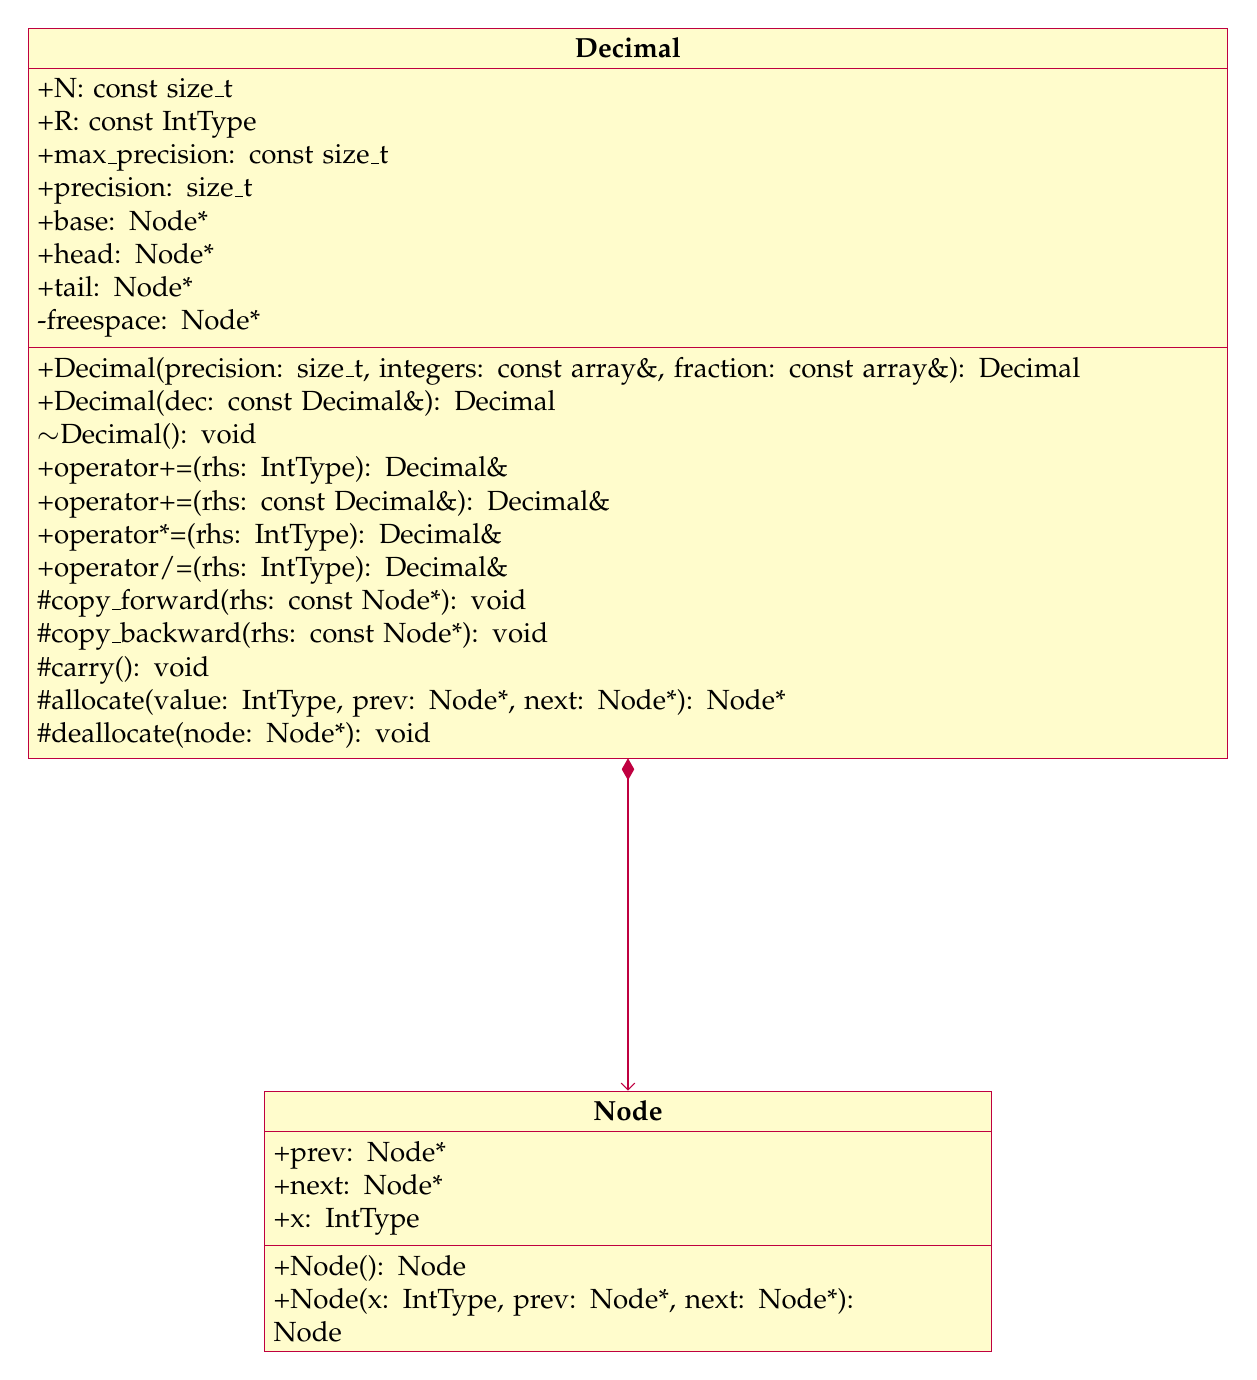
\begin{tikzpicture}
    \begin{class}[text width=15cm]{Decimal}{0,0}
    	\attribute{+N: const size\_t}
    	\attribute{+R: const IntType}
        \attribute{+max\_precision: const size\_t}
        \attribute{+precision: size\_t}
        \attribute{+base: Node*}
        \attribute{+head: Node*}
        \attribute{+tail: Node*}
        \attribute{-freespace: Node*}
        \operation{+Decimal(precision: size\_t, integers: const array\&, fraction: const array\&): Decimal}
        \operation{+Decimal(dec: const Decimal\&): Decimal}
        \operation{$\sim$Decimal(): void}
        \operation{+operator+=(rhs: IntType): Decimal\&}
        \operation{+operator+=(rhs: const Decimal\&): Decimal\&}
        \operation{+operator*=(rhs: IntType): Decimal\&}
        \operation{+operator/=(rhs: IntType): Decimal\&}
        \operation{\#copy\_forward(rhs: const Node*): void}
        \operation{\#copy\_backward(rhs: const Node*): void}
        \operation{\#carry(): void}
        \operation{\#allocate(value: IntType, prev: Node*, next: Node*): Node*}
        \operation{\#deallocate(node: Node*): void}
    \end{class}
    \begin{class}[text width=9cm]{Node}{0,-13.5}
    	\attribute{+prev: Node*}
    	\attribute{+next: Node*}
    	\attribute{+x: IntType}
    	\operation{+Node(): Node}
    	\operation{+Node(x: IntType, prev: Node*, next: Node*): Node}
    \end{class}
    \composition{Decimal}{}{}{Node}
\end{tikzpicture}
\caption{Decimal类图}
\end{figure}

\subsection*{四、使用说明、测试分析与结果}
\subsubsection*{1、使用说明}
1) 请使用支持C++14及以上标准的编译器生成目标文件。 \par
2) 进入程序后依照需求的输入样式输入数据,手动输入与流式输入都是被允许的。 \par
3) 计算十万位$\pi$值的耗时将达到一分钟。除非您清楚您在做什么,否则不建议输入过大的数,以免造成不必要的时间浪费。 \par
4) 为了防止终端卡死,当期望精度较大时,比较推荐的做法是将输出结果重定向写入文件。 \par
5) 如果你希望使用Decimal类,请在您的代码中注明出处。关于大数类的接口请阅读源码相关注释,并参考已提供的计算$\pi$值的代码以便快速使用该类。

\subsubsection*{2、测试结果与分析}
2.1\;\textbf{实际环境} \par
以$\mathbf{Algorithm\;1}$提供的$\pi$值计算方法为目标,输入操作数的范围约束在正整数,满足实现的大数计算子集Decimal类。但是持续的迭代将最终导致操作数越过方法所能支持的计算范围,造成结果溢出。Decimal不计划对已实现的方法放松输入约束,故该情景应由用户合理处理以满足约束。\par
2.2\;\textbf{边界情况} \par
1) 输入精度为0 \par
2) 导致被除数为0的Divide操作数 \par
3) 导致被乘数出现后缀0的Multiply操作数 \par
4) 约束范围内最大值的Multiply操作 \par
2.3\;\textbf{测试结果} \par
1) 问题期望输出:3,算法期望输出:2,实际输出:2 \par
\textbf{问题分析:} 实际输出满足算法的期望输出,与问题的期望输出的差异源于Decimal类计算流程的内在逻辑。 \par
\textbf{解决办法:} 输出结果符合算法逻辑,不考虑为程序漏洞。若有纠正的需求,应由Decimal类的使用者适配需求具体化处理。 \par
2) 期望输出:0,实际输出:陷入死循环 \par
\textbf{问题分析:} 目标代码未考虑该种情况。当除法结果为零时,未及时清除后缀零并重置当前精度,导致当前Decimal类数据非法,干扰后续方法的执行逻辑,陷入死循环。 \par
\textbf{解决办法:} 根据$\mathbf{Algorithm\;4}$给出的算法流程,可以断言当尾项除法结果为零时,该Decimal被除为0。故在除法流程结束后,基于此断言追加特判以将当前Decimal重置为0。 \par
3) 样例输入:Multiply(3.14, 5), N=1, max\_precision=2 \par
\;\;\;\;\,期望输出:15.7,错误期望输出:15.70,实际输出:15.7
\par
\textbf{问题分析:} 基于$\mathbf{Algorithm\;4}$给出的算法流程,目标代码的具体实现在乘法过程结束后追加了抹除整数部分前导零的操作,实际输出符合期望。 \par
4) 样例输入:Multiply(9999999999.9999999999, 9999999999), N=10, sizeof(IntType)=8bytes \par
\;\;\;\;\,期望输出:99999999989999999999.0000000001,实际输出:776627961-2066097414.1452241921 \par
\textbf{背景引入:} 目标代码的实现使用了C++模板以约束IntType与参数N的关系,在源代码逻辑中,作出了以下断言:若$10^{2N}>IntType::max()$,则模板参数对(IntType,N)将会导致计算过程的结果溢出。 在该种情况下,目标代码将会被否决并使编译过程强制失败。\par
\textbf{问题分析:} 其一,断言的判定基于$10^{2N}$的计算,其本身也是有限位长的数,溢出的情况依旧存在。源代码提供的$10^{2N}$模板值计算并未校验其本身的正确性,导致最后的断言结果出现差错。其二,经过重新分析发现,$10^{2N}$并非计算过程的理论最大值。Decimal计算流程的最大值出现在Multiply方法,取所有输入为上限值,则单项乘法的最大值为$(10^N-1)^2$,而进位将会额外提供最大为$\lfloor\frac{(10^N-1)^2}{10^N}\rfloor$的加数。N的范围被约束在正整数,故可得计算过程的实际理论最大值为$10^{2N}-10^N-1$。该值的误差对断言的正确性亦造成了一定的干扰。 \par
\textbf{解决办法:} 其一,引入新的Check模板ispow10\_t<target>以判定相关计算结果$10^N$,$10^{2N}$是否正确。若错误,则可断言过程存在溢出情况。其二,计算过程理论上限纠正为$10^{2N}-10^N-1$。 \par

\subsubsection*{3、设计与实现的回顾讨论与分析}
对于相对复杂的目标,在编码之前进行模糊或清晰的设计就尤为重要。而相较于高耦合的代码,高内聚低耦合的结构则更易于调试与优化。计算$\pi$值的程序并不复杂,单纯为了实现计算目标进行编码,大致可以在200行之内完成。但是相对应的,若是出现了预料之外的错误,糅杂在一起、彼此密切关联的代码就显得难以调试。 \par
故出于易于调试、优化以及一定程度上的拓展考虑,对此实验我选择单独实现大数类并引入模板以便静态检查等操作。 \par
考虑到完全实现的复杂性与针对问题的无用性,源代码只实现了大数相加,大数-定长整形加法,大数-定长整形乘法,大数-定长整形除法四项算术操作。而从最终的$\pi$值计算主程序可以得出,这个决定是正确的。源代码实现的任意一个方法都被有效使用,且主程序的编码复杂度几乎为0。 \par
针对编码过程中出现的一些问题,皆可以对应到独立的方法或者代码块,而无需在逻辑链条上多处修改。 \par
对于大数类的存储结构,Decimal选择了由$(head,base,tail)$三个节点引导组成的双链表,其中head指引最高位单元,base指引整数部分的第一个单元,而tail则指引最低单元。base的存在定位了小数点,而head,tail则使得两端易于访问,分别加速了Divide与Multiply的过程。针对除法不可除尽的情况,该类选择实现的是大数,而不是高精度。两者的区别在于除法操作是否无损。出于精度问题考虑,Decimal引入了max\_precision与precision成员用以指示除法步骤的最大迭代次数。而对于计算$\pi$值,precision的引入恰恰又解决了何时停止迭代的问题。令max\_precision为期望精度,则precision达到max\_precision并在进入下一轮时,计算增量被除为0,precision重置,此时也即计算的$\pi$不再改变,这同样也意味着期望的精度已经满足,可以终止迭代。 \par
平心而论,以Decimal类作为$\pi$计算的中介会带来必然的性能损失。但是从可读性、可维护性衡量,这样的交易是利大于弊的。

\subsubsection*{4、运行界面}
\begin{figure}[H]
	\begin{minipage}[t]{\linewidth}
		\centering
		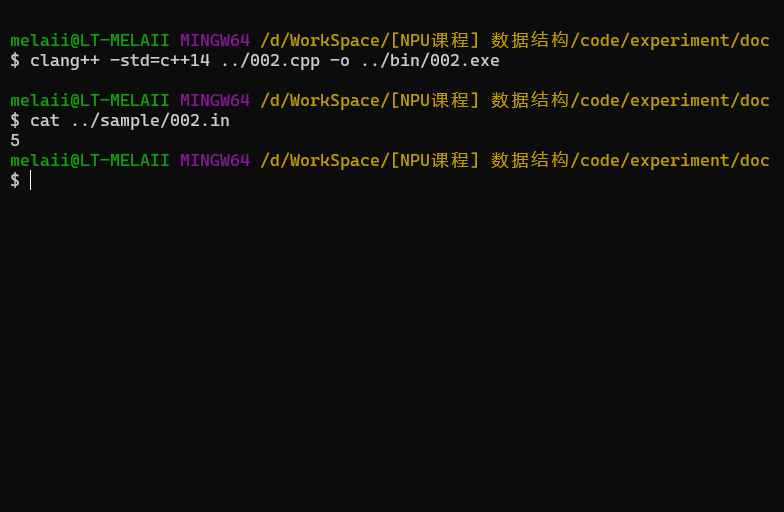
\includegraphics[width=125mm,height=80mm]{./assets/DS02-2}
		\caption{前置环境}
	\end{minipage}
\end{figure}
\begin{figure}[H]
	\begin{minipage}[t]{\linewidth}
		\centering
		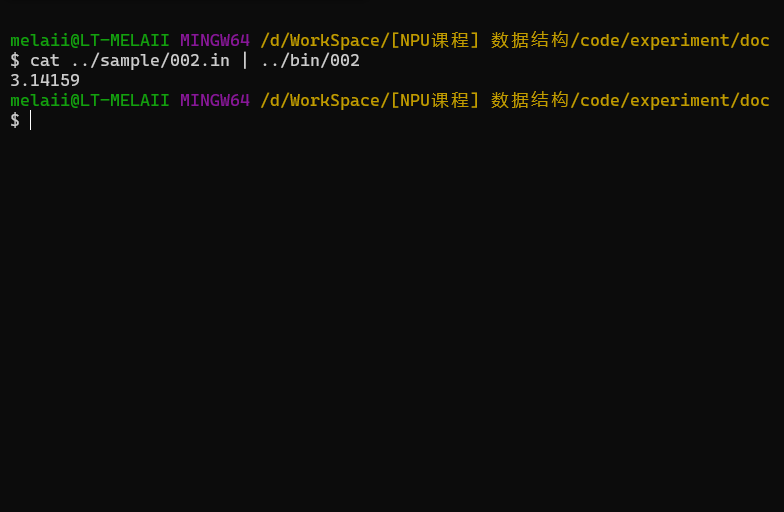
\includegraphics[width=125mm,height=80mm]{./assets/DS02-3}
		\caption{结果输出}
	\end{minipage}
\end{figure}
\begin{figure}[H]
	\begin{minipage}[t]{\linewidth}
		\centering
		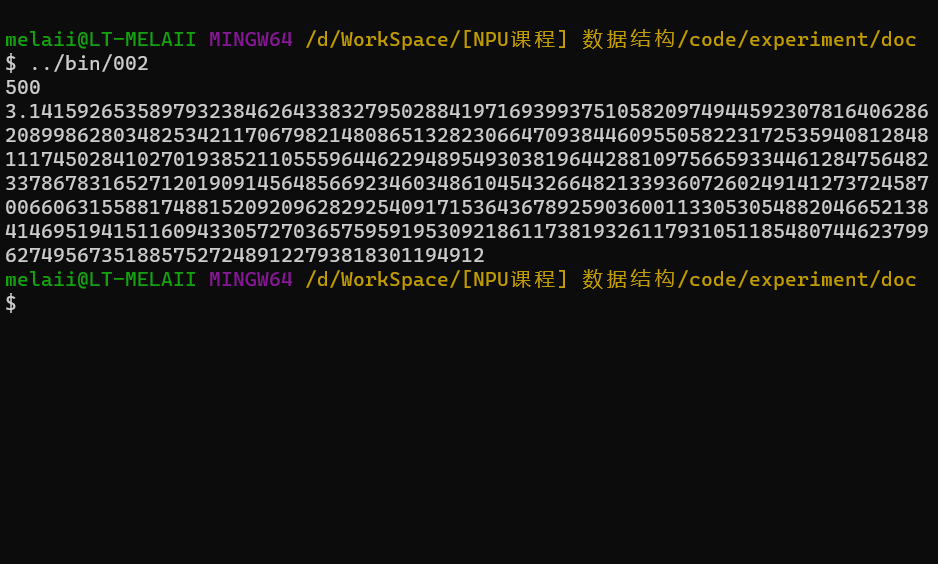
\includegraphics[width=125mm,height=80mm]{./assets/DS02-4}
		\caption{500位精度输出}
	\end{minipage}
\end{figure}

\subsection*{五、实验总结}
熟练使用双链表是该实验的基础,而基于双链表实现大数计算则是该实验的应用点。考虑清楚如何计算$\pi$以及如何计算大数这两个问题,整个实验过程也可以提前告终,剩下的时间则是留给了编码与测试-调试-优化的迭代过程。 \par
对于我来说,该实验的重点在于优化。本文提供的四个算法是流程概述,但是一板一眼的根据其实现,这样的代码写出来也会有大量的优化空间。 \par
基于我所选择的存储形式,在算法不变的前提下,我为定最大的优化空间在于0的处理与内存分配的处理。0的处理,也即计算过程带来的无用前导0与后缀0,两者在任意情况下都是没有意义的,故在Decimal的维护中,我选择在会产生这两种情况的过程之后擦除前后缀0。而由此自然而然带来的问题就是被擦除的0所在的节点该何去何从。对于计算密集的Decimal应用,这将带来频繁的内存释放与申请,故不妨将内存释放的操作延迟到对象析构,在每次擦除节点时,将该节点存入空闲节点链表。若存在空闲节点,则直接从其中分配。对于0的问题还存在另一个优化空间,也即除与模操作在该情境下的必要性。虽则没有性能分析的优化都是胡闹,但是除模指令损耗的时钟周期长是不争的事实。故我在逻辑判断的损耗优于除模指令的假定前提下,选择直接跳过0值项的计算步骤。 \par
关于最终的实验结果,仅根据NOJ差劲的评测系统给出的数据反馈,Decimal在内存上的表现是优秀的,而性能在横向比较上也处在不差的地位。 \par
总而言之,对于该实验的整体代码实现我是满意的。在使用双向链表这个大前提下,代码可读性、结构划分和性能表现都不差。满意于自己的成果,我想最大的收获也莫过于此了吧。

~\\
\zihao{-4}
\textbf{教师评语:}
~\\
\textbf{实验成绩:}

\begin{flushright}
\mbox{指导教师签名:\qquad\qquad} \\
\mbox{批阅日期:\qquad\qquad}
\end{flushright}

\end{document}